\documentclass{standalone}
\usepackage{tikz}
\usepackage{amssymb}

\begin{document}
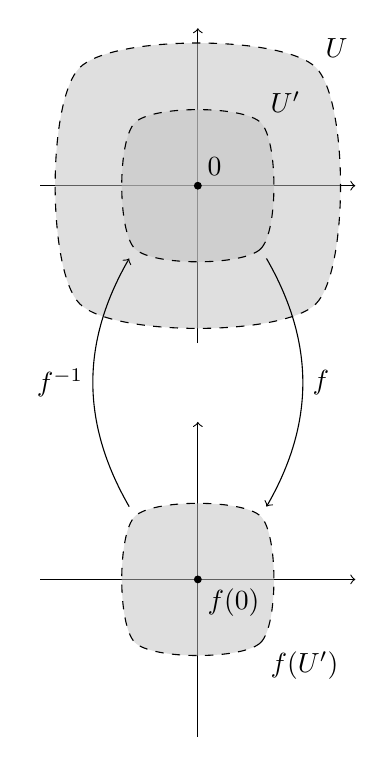
\begin{tikzpicture}
  \draw[->] (-2,0) -- (2,0);
  \draw[->] (0,-2) -- (0,2);

  \filldraw[dashed, fill=gray!50, fill opacity=0.5] plot[smooth cycle]
    coordinates {(-1.5,-1.5) (1.5, -1.5) (1.5, 1.5) (-1.5, 1.5)};
  \node at (1.5, 1.5) [above right] {$ U $ };

  \filldraw[dashed, fill=gray!50, fill opacity=0.5] plot[smooth cycle]
    coordinates {(-0.8,-0.8) (0.8, -0.8) (0.8, 0.8) (-0.8, 0.8)};
  \node at (0.8, 0.8) [above right] {$ U' $};

  \fill (0,0) circle (0.05);
  \node at (0,0) [above right] {$ 0 $};

  \node at (0.8, -0.8)(a){};
  \node at (-0.8, -0.8)(b){};

  \begin{scope}[yshift=-5cm]
    \draw[->] (-2,0) -- (2,0);
    \draw[->] (0,-2) -- (0,2);

    \filldraw[dashed, fill=gray!50, fill opacity=0.5] plot[smooth cycle]
      coordinates {(-0.8,-0.8) (0.8, -0.8) (0.8, 0.8) (-0.8, 0.8)};
    \node at (0.8, -0.8) [below right] {$ f(U') $};

    \fill (0,0) circle (0.05);
    \node at (0,0) [below right] {$ f(0) $};

    \node at (0.8, 0.8)(c){};
    \node at (-0.8, 0.8)(d){};
  \end{scope}
  
  \draw[bend left, ->] (a) to node[right]{$ f $} (c);
  \draw[bend right, <-] (b) to node[left]{$ f ^{-1} $} (d);

\end{tikzpicture}
\end{document}
